\chapter{Algoritmi Greedy}
Si tratta di una tecnica che si applica sempre ai problemi di ottimizzazione, ma
rispetto alla programmazione dinamica ha un approccio diverso, dato che il calcolo della
soluzione ottima (in questo caso ne calcola una sola) avviene attraverso una
sequenza di scelte \textbf{localmente} ottime.
\paragraph*{Caratteristiche degli algoritmi Greedy}
\begin{itemize}
    \item Semplici da scrivere
    \item Efficienti
\end{itemize}
\paragraph*{Questioni}
\begin{itemize}
    \item Dimostrare la correttezza di un algoritmo greedy
    \item Capire quali problemi sono affrontabili con una strategia greedy
\end{itemize}
\section{Problema - Selezione attività}
\paragraph*{INPUT} Dato un insieme $A = \{a_1, a_2, \dots, a_n\}$ di n attività, tale
che $a_i = [s_i, e_i)$ per $\ \leq i \leq n$, dove $s_i$ è il tempo di inizio ed $e_i$ è il
tempo di fine.
\begin{center}
    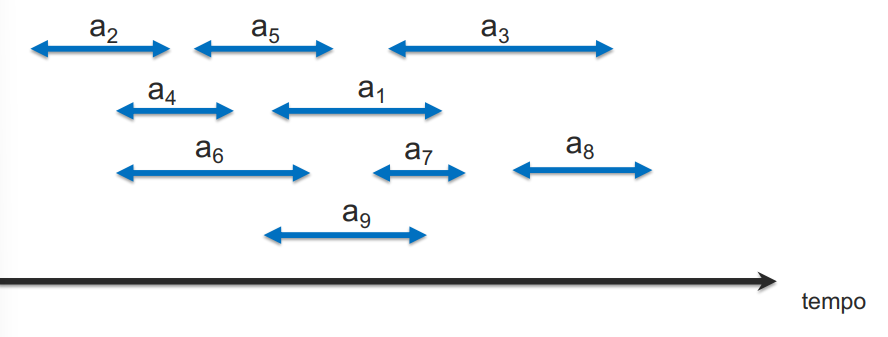
\includegraphics[width=80mm,scale=0.5]{greedy_sel_attivit.png}
\end{center}
$a_i=[s_i, e_i)$ e $a_j = [s_j, e_j)$ sono \textbf{compatibili} se $s_i \geq e_j$ oppure 
$s_j \geq e_i$. In poche parole se un attività inizia nello stesso momento della fine dell'altra, oppure dopo.
Le attività non devono accavallarsi, cioè eseguirsi nello stesso tempo di un'altra.
Facciamo qualche esempio che sicuramente è più semplice.\\
Per esempio $a_5=[s_5, e_5)$ e $a_8 = [s_8, e_8)$ sono compatibili, mentre $a_5 = [s_5, e_5)$ e 
$a_1 = [s_1, e_1)$ NON sono compatibili, infatti l'inizio di $a_1$ è minore della fine di $a_5$.
\paragraph*{OUTPUT} il sottoinsieme X di cardinalità massima composto di attività mutuamente compatibili.
In questo esempio l'OUTPUT desiderato è $X = \{a_2, a_5, a_7, a_8\}$.
\subsection{Soluzione con DP}
$A = \langle a_1, a_2,\dots,a_n\rangle$ tale che $e_1 \leq e_2 \leq \dots \leq e_n$.\\
$A = A \cup \{a_0, a_{n+1}\} = \langle a_0, a_1, \dots, a_n, a_{n+1}\rangle$ tale che $e_0 \leq s_1$
e $s_{n+1} \geq e_n$.
\paragraph*{Sottoproblema (i,j) per $0 \leq i < j \leq n+1$}
Trovare il sottoinsieme $X_{ij}$ di attività mutuamente compatibili di cardinalità massima per
$A_{ij} = \langle a_{i+1}, a_{i+2},\dots,a{j-2}, a{j-1} \rangle$.
\paragraph*{Sottoproblema $(0, n+1)$}
Trovare il sottoinsieme $X_{0,n+1} = X$ di attività mutuamente compatibili di cardinalità
massima per $A_{0,n+1} = \langle a_1, a_2, \dots, a_{n-1}, a_n \rangle = A$.\\
Numero totale di sottoproblemi \ra $(n+1)+n+(n-1)+(n-2)+\dots+1$.
\paragraph*{CASI BASE per $j=i+1 (A_{ij}=\emptyset)$}
$X_{ij} = \emptyset$.
\paragraph*{PASSO RICORSIVO per $j > i +1 (A_{ij} \neq \emptyset)$}
\textbf{Sottostruttura ottima}\\
$a_k$ appartiene a $X_{ij} \implies X_{ij} = X_{ik} \cup \{a_k\} \cup X_{kj}$\\
$X_{ik}$ soluzione ottima di $A_{ik}$\\
$X_{kj}$ soluzione ottima di $A_{kj}$\\
$X_{ij} = max\{X_ik \cup \{a_k\} \cup X_kj \text{ per } i < k < j\}$.
\paragraph*{Valore ottimo - Sostituzione coefficiente all'eqauzione}
\paragraph*{CASI BASE per $j=i+1 (A_{ij}=\emptyset)$}
$c_{ij} = 0$ (valore ottimo)
\paragraph*{PASSO RICORSIVO per $j > i +1 (A_{ij} \neq \emptyset)$}
$c_{ij} = max\{c_{ik} + 1 + c_kj \text{ t.c } i < k < j\}$ (valore ottimo).
\subsection{Svantaggi della Soluzione tramite DP}
\begin{enumerate}
    \item Tutti i sottoproblemi devono essere risolti per arrivare a calcolare il valore ottimo
    \item Si deve in seguito ricostruire la soluzione ottima (soluzione ottimale) perchè io ho solo
    i coefficienti, non ho la sequenza richiesta in OUTPUT
\end{enumerate}
\subsection{Approccio greedy}
\begin{center}
    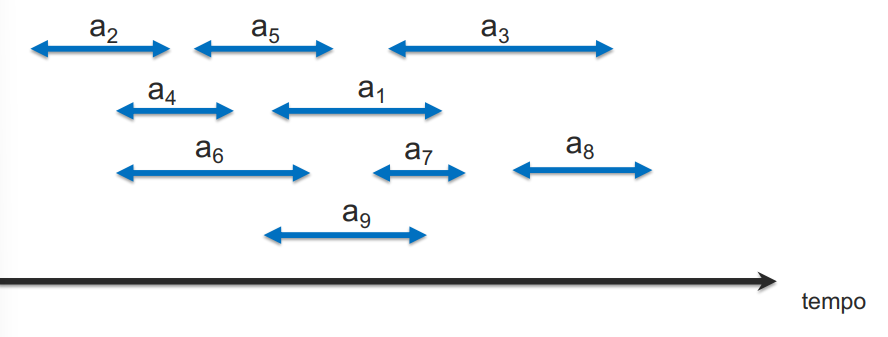
\includegraphics[width=80mm,scale=0.5]{greedy_sel_attivit.png}
\end{center}
In questo caso dobbiamo scegliere un parametro, per esempio \ra Attività con il tempo
di fine più basso, che in questo caso è $a_2$.\\
\textbf{IPOTESI}: $a_2$ appartiene alla soluzione ottima X $\implies X = \{a_2\} \cup X_2$.\\
\textbf{$X_2$ è la soluzione ottima per $A_2 = \{a = [s,e) \in A | \text{ a compatibile con } a_2\}$}
Compatibile con $a_2$ significa che $s \geq e_2$. Graficamente devo avere che la fine di $a_2$ non si
intersechi nessuna attività. Quindi devo cercare l'attività con il tempo di fine più basso in $A_2 \rt a_5$.
\begin{center}
    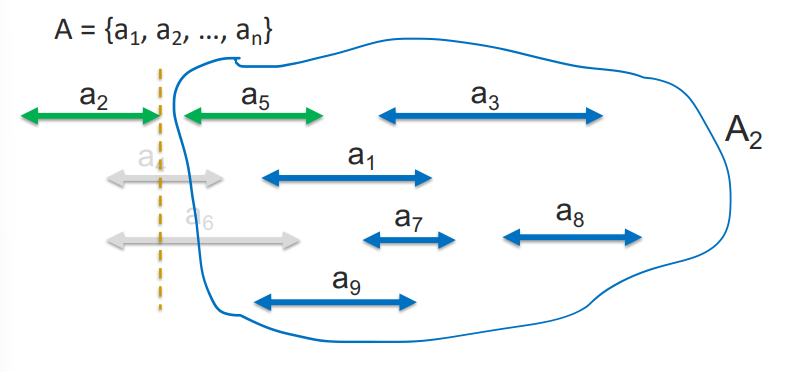
\includegraphics[width=80mm,scale=0.5]{greedy_sel_attivit_p2.png}
\end{center}
Scelgo quindi $a_5$ dato che ha il tempo di fine più basso rispetto a tutte le attività 
compatibili con $a_2$.\\
\textbf{IPOTESI} $a_5$ appartiene alla soluzione ottima $X_2 \implies X = \{a_2\} \cup \{a_5\} \cup X_2$.\\
$X_5$ è soluzione ottima per $A_5 = \{a=[s,e) \in A | s \geq e_5\}$.\\
Ancora una volta cerco le attività compatibili con $a_5$, che abbiano quindi un inizio che sia maggiore
o uguale rispetto alla fine di $a_5$, e scelgo quella con tempo di fine minore.\\
Determino quind che $A_5 \rt a_7$.\\
\textbf{IPOTESI}: $a_7$ appartiene alla soluzione ottima $X_5 \implies X = \{a_2\} \cup \{a_5\} \cup \{a_7\} \cup X_7$.\\
Cerco nuovamente l'attività con tempo di fine più basso rispetto a quelle compatibili con $a_7$ e trovo
che l'attività in questione è $a_8$.\\
\textbf{IPOTESI}: $a_8$ appartiene alla soluzione ottima $X_7$.\\
Quindi questo implica che $X = \{a_2\} \cup \{a_5\} \cup \{a_7\} \cup \{a_8\} \cup X_8$.\\
$X_8$ è soluzione ottima per $A_8 = \{a=[s,e) \in A\,t.c\, s \geq e_8\}$.\\
Ma dato che non ho più eventi compatibili con $a_8$ (perchè sono finiti, ma valeva anche il caso che c'erano altri
eventi che NON compatibili), $A_8 = \emptyset$. Significa che sono arrivato ad avere la soluzione
e guardandola notiamo che è una soluzione ottimale.\\
\[ X = \{a_2, a_5, a_7, a_8\} \]
\subsection{Osservazioni sulla risoluzione Greedy}
Notiamo che ad ogni passo la scelta localmente ottima minimizza il tempo di fine. Sono state effettuate
4 scelte localmente ottime, sono quindi stati risolti 4 sottoproblemi.\\
\paragraph*{In sintesi} Ad ogni passo:
\begin{enumerate}
    \item effettuo una scelta localmente ottima
    \item risolvo il sottoproblema generato dalla scelta appena effettuata
    \item la scelta non dipende dalle scelte successive (Greedy è anche detto algoritmo miope)
    \item la scelta riduceo il sottoproblema da risolvere (approccio Top-Down)
\end{enumerate}
\subsection{Codice Greedy}
\begin{lstlisting}[language=Java, escapeinside={*@}{@*}]
    Procedura greedy_scheduling(A)
        n = |A|
        *@$a_s$@* = attivita' di A con il minore tempo di fine
        X = {@*$a_s$@*}
        @*$a_s$*@ = a=[s,t) t.c @*$s \geq e_s$@* e minore tempo di fine
        while @*$a_s \neq NIL$*@ do
            X = @*$\{a_s\} \cup X$*@
            @*$a_s$*@ = a=[s,t] t.c @*$s \geq e_s$*@ e minore tempo di fine
        return X
\end{lstlisting}
Tempo di esecuzione $O(n)^2$, determinato dal While, perchè le altre
operazioni o sono costanti o nel caso della ricerca dell'evento compatibile
con tempo di fine minore impiegano tempo $O(n)$.
\paragraph*{Miglioramento} Posso migliorare l'algoritmo ordinando le attività di A per tempo di fine
non decrescente,
prima di eseguire le operazioni di ricerca evento minimo, inserisco quindi un
tempo di $O(n\log n)$ determinato dall'algoritmo di ordinamento (es. MergeSort o QuickSort).\\
Dopodichè aggiungo $a_1$ alla soluzione ottima di X, dato che sarà sicuramente l'attività minore (visto
che le ho ordinate). Aggiungo 

